\chapter{Etat de l'art}

\paragraph{}
Ce projet consiste en la réalisation d'un module noyau pour FreeBSD rendant
possible l'utilisation d'un volume chiffré avec
\textit{LUKS}\cite{onDiskFormatLuks}, un standard de chiffrement associé au
noyau Linux.
\paragraph{}
L'objectif est donc de relever et comparer les moyens de chiffrement de disques
actuels, et d'analyser plus particulièrement les modules noyau Linux et FreeBSD
gérant le chiffrement de volume afin de porter le standard
\textit{LUKS}\cite{onDiskFormatLuks} vers FreeBSD.

\section{Différents niveaux de chiffrements}

\subsection{Chiffrement à la volée}
\paragraph{}
Le chiffrement de disque est généralement géré par le noyau du système, ou par
des logiciels spécialisés comme TrueCrypt ou VeraCrypt sur Windows. Il permet de
chiffrer et déchiffrer des partitions entières à la volée. Le disque, une fois
déchiffré, peut-être montré comme n'importe quel autre espace de stockage. Son
utilisation est totalement transparente pour l'utilisateur.
\paragraph{}
Dans des systèmes comme Linux ou FreeBSD, le chiffrement et déchiffrement du
disque est réalisé directement par le noyau. Au moment de la lecture et de
l'écriture du disque, les données passent par une couche supplémentaire
(\textit{dm-crypt} pour Linux et \textit{GELI}\cite{manGeli} pour FreeBSD) dont
le rôle est de faire le lien entre les données chiffrées du disque et celle en
claire visibles et utilisables par l'utilisateur.
\paragraph{}
Le fait que la lecture d'un disque soit faite par le noyau permet à un système
utilisant cette méthode de chiffrer tout le système, à l'exception d'une petite
partie permettant de déchiffrer le noyau au démarrage. Le reste du système peut
ensuite être directement déchiffré par le noyau.

\subsection{Chiffrement au niveau du système de fichiers}
\paragraph{}
Le chiffrement de système de fichier consiste en la création d'un système de
fichier qui sera ensuite enregistré chiffré sur le disque. C'est nottament la
technoligie utilisée par l'\textit{Encrypting File System} (abrégé EFS), une
technologie Microsoft disponible dès la troisième version des systèmes de
fichiers NTFS. D'autres solutions existent également, comme EncFS. Des logiciels
comme TrueCrypt/VeraCrypt permettent également de réaliser de genre
d'opérations, en chiffrant des fichiers dans un conteneur.
\paragraph{}
Le type de chiffrement a l'avantage de chiffrer toute une arborescence de
fichiers indépendamment des autres fichiers présents sur le disque. Cela permet
d'avoir différentes clés de chiffrement par système de fichiers chiffrés,
contrairement au chiffrement de disque qui en impose une seule par partition.
\paragraph{}
Ce type de chiffrement peut cohabiter sur un système utilisant déjà le
chiffrement de disque. Il ne permet en revanche pas de chiffrer des fichiers
nécessaires au démarrage du système, contrairement à l'autre type de
chiffrement.

\subsection{Chiffrement de fichier}
\paragraph{}
Ce type de chiffrement permet de chiffrer un seul fichier. Il peut s'agir
d'archives possédant cette propriété de pouvoir être chiffrées et déchiffrées
par les logiciels spécialisés. Dans ce cas, seul le contenu de l'archive est
chiffré et les métadonnées restent en clair. C'est le type de chiffrement
utilisé par des archives comme \textit{7z}. Le chiffrement peut également se
faire directement sur un fichier, en utilisant des solutions comme
\textit{gpg}, en créant un nouveau fichier \textit{.gpg} étant le chiffré de
celui d'origine.

\subsection{Chiffrement matériel}
\paragraph{}
Le chiffrement matériel (\textit{Hardware-based full disk encryption},
\textit{FDE}) concerne certains disques (appelés \textit{Self-encrypting drive})
ou autres espaces de stockage. Leur fonctionnement est basé sur le contrôleur
qui gère les clés de chiffrement servant au chiffrement du disque, et
œuvrant indépendamment du processeur. L'authentification se fait alors avec un
via un logiciel s'exécutant avant le démarrage du système ou mot de passe dans
le BIOS.
\paragraph{}
Le groupe \textbf{Trusted Computing Group} réunissant plusieurs fabricant a mis
en place une spécification, \textit{Opal Storage Specification}, pour ce type de
disques auto-chiffrés.

\section{Chiffrement de disque sur Linux et FreeBSD}

\paragraph{}
Le chiffrement de disque sous Linux et FreeBSD est un chiffrement à la volée. Il
est géré par des modules noyaux qui interviennent au moment de la lecture et
l'écriture du disque. Les opérations qu'ils réalisent sont totalement
transparentes du point de vue de l'utilisateur, qui ne manipule que des données
en clair.
\paragraph{}
Chacun des deux systèmes a accès à différents algorithmes implémentés dans le
noyau et permettant le hachage et la chiffrement de données. Le chiffrement sur
les deux systèmes peut se faire sur des disques entiers, des partitions
physiques ou logiques (comme LVM), des volumes RAID, la RAM, ...
\paragraph{Linux}
Le module permettant de manipuler un disque chiffré sous Linux se nomme
\textit{dm-crypt}. Ce module a été ajouté à l'infrastructure
\textit{device-mapper} à la version 2.6 du noyau.\\
\\
Le standard qui est actuellement le plus utilisé pour le chiffrement de disque
est \textit{LUKS} (\textit{Linux Unified Key Setup}\cite{onDiskFormatLuks}). Son
rôle est de chiffrer intégralement un volume tout en le rendant utilisable par
d'autres plate-formes.
\paragraph{FreeBSD}
Le module permettant cette opération sous FreeBSD se nomme \textit{GELI},
remplaçant l'ancien module \textit{GBDE}. Il appartient à la classe
\textit{GEOM}, qui contient l'ensemble des modules permettant de manipuler des
disques et autres volumes.\\
\\
Contrairement à \textit{dm-crypt} qui peut accepter des paramètres correspondant
à différents standards (non limités à LUKS), le seul standard disponible pour
le chiffrement de volume avec \textit{GELI} est celui ce \textit{GELI} lui-même.

\subsection{Organisation dans le système d'exploitation}
\paragraph{}
Dans le cas de {\em Linux}, le chiffrement de disque est géré par le module 
noyau {\em dm-crypt}, qui est un module qui dépend du module plus général
{\em device-mapper} qui gère les transformations de disque sous {\em Linux} 
(RAID, LVM, Cache, ...).
Le module {\em dm-crypt} gère la table appelée {\em crypt table}
qui permet d'associer un device à un chiffrement notamment. La table permet
la lecture des données sur le disque. À celà s'ajoute le programme 
{\em cryptsetup} qui permet de lire des métadonnées stockées sur le disque 
pour remplir la {\em crypt table}.
Le programme s'occupe notamment du déchiffrement de la clé, de 
la lecture et de l'écriture des métadonnées sur le disque. L'organisation est 
donc la suivante :

\paragraph{}
\begin{figure}[h]
\centering
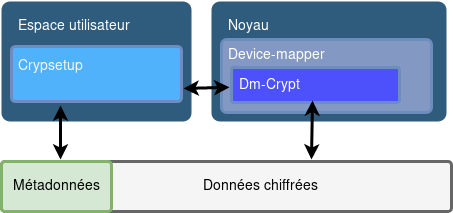
\includegraphics[width=.8\linewidth]{etat_art/organisation_linux.png}
\caption{\label{fig:OrgLinux}Organisation du code dans Linux}
\end{figure}

\paragraph{}
L'organisation reflétée par les programmes l'est également au niveau du code,
le module {\em dm-crypt} est agnostique de l'existance de métadonnées ainsi 
que de leur format. On a donc le module {\em device-mapper \em et \em dm-crypt}
qui font partie du code du noyau {\em Linux}, tandis que {\em Crypsetup} est un 
programme qui est usuellement fourni avec {\em Linux} en tant qu'utilitaire, 
qui est géré par une équipe indépendante de celle du noyau {\em Linux}. De plus 
{\em dm-crypt} est agnostique des algorithmes de chiffrement disponibles,
le module s'appuie sur l'API de cryptographie du noyau.

\paragraph{}
Dans le cas de {\em FreeBSD}, le module noyau qui est en charge des
transformations sur les disques est {\em GEOM}. Comme sous {\em Linux}, 
il existe des modules qui vont interagir avec {\em GEOM} pour fournir des 
fonction de RAID, de cache, et également de chiffrement. 
Ces modules sont appelés {\em Classes GEOM}, 
celle qui fournit le chiffrement est nommée {\em ELI}, le module noyau associé 
est ainsi appelé {\em GELI}. Le module contrairement à {\em dm-crypt}, 
comprend toute la logique des métadonnées, ainsi que des algorithmes de 
chiffrement disponibles. L'outil en espace utilisateur tire son code
directement du code du module {\em geli}. {\em GELI} profite de la 
connaissance du format des métadonnées pour directement détecter les 
partitions chiffrées, et donc proposer leur déchiffrement à l'utilisateur, 
là où {\em Linux} ne peut pas détecter de
partition ou disque chiffré, et c'est à l'utilisateur de préciser qu'il veut 
déchiffrer tel disque avec l'outil {\em crypsetup} qui va donc reconnaître le 
format. On a donc l'organisation suivante :


\paragraph{}
\begin{figure}[h]
\centering
\includegraphics[width=.8\linewidth]{etat_art/organisation_FreeBSD.png}
\caption{\label{fig:OrgFreeBSD}Organisation du code dans FreeBSD}
\end{figure}

\subsection{Format sur disque}
\paragraph{}
Le format sur disque désigne l'organisation des données et métadonnées sur le 
disque. L'idée générale étant de stocker sur une partie du disque les 
informations permettant de déchiffrer une autre partie du disque.
\paragraph{}
Comme le noyau {\em Linux} ne contient pas de format de métadonnées, 
c'est {\em Crypsetup} qui a choisi de créer un format appelé {\em Linux 
Unified Key Setup ({\em LUKS})}, comme format standard pour le chiffrement de 
disque sous {\em Linux}. En effet, {\em Crypsetup} implémente d'autres format 
de métadonnées comme {\em TrueCrypt} développé par la 
{\em TrueCrypt Fondation}. 
Le format {\em LUKS} consiste en des métadonnées au début de la partition, 
précédant les données chiffrées.

\paragraph{}
\begin{figure}[h]
\centering
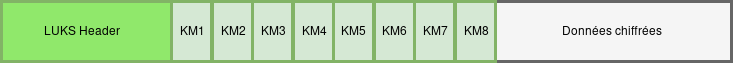
\includegraphics[width=.8\linewidth]{etat_art/format_disque_luks.png}
\caption{\label{fig:LUKSFormat}Format sur disque LUKS}
\end{figure}

\paragraph{}
Les métadonnées de {\em LUKS} contenant les algorithmes de chiffrement, 
d'authentification, la version de {\em LUKS}, sont suivis de huit emplacements 
permettant de stocker des clés chiffrées, qui permettent de déchiffrer le 
disque. Ainsi on peut stocker la même clé huit fois, protégées par des mots de 
passe différents, permettant ainsi à plusieurs utilisateurs de déchiffrer le 
même disque sans pour autant partager le même mot de passe.

\paragraph{}
Les métadonnées de {\em GELI} sont stockées contrairement à {\em LUKS}, 
à la fin du disque.
L'en-tête permet de stocker 2 clés, et s'étend sur un seul secteur.


\paragraph{}
\begin{figure}[h]
\centering
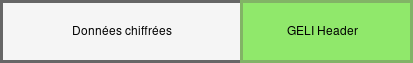
\includegraphics[width=.5\linewidth]{etat_art/format_disque_geli.png}
\caption{\label{fig:GELIFormat}Format sur disque GELI}
\end{figure}

\paragraph{}
Dans les deux en-têtes on retrouve des champs similaires, un {\em Magic} qui 
permet de connaître le type d'en-tête, la version, l'algorithme de chiffrement 
et d'authentification, etc. On peut noter tout de même que la taille de 
l'en-tête sous {\em GELI} fait 255 octets, contre 592 octets pour {\em LUKS}.



\subsection{Algorithmes}
\subsubsection{Algorithmes de chiffrement}
\paragraph{}
Les algorithmes de chiffrement disponibles pour {\em GELI} \cite{geli.h} sont :
\begin{itemize}
	\item Null
	\item Null-CBC
	\item AES-CBC
	\item AES-XTS
	\item Blowfish
	\item Blowfish-CBC
	\item Camellia
	\item Camellia-CBC
	\item 3DES
	\item 3DES-CBC
\end{itemize}

\paragraph{}
Dans le cas de {\em LUKS}, la spécification \cite{onDiskFormatLuks}
la liste des algorithmes disponibles, les noms des algorithmes ne sont pas 
interprétés par des opérations {\em LUKS}, mais pour des besoins de 
compatibilité avec d'autres implémentations, la liste des algorithmes 
disponibles est la suivante :
\begin{itemize}
	\item AES
	\item Twofish
	\item Serpent
	\item Cast5
	\item Cast6
\end{itemize}
Les algorithmes peuvent être associés aux modes suivants :
\begin{itemize}
	\item ECB
	\item CBC-plain
	\item CBC-essiv:hash
	\item XTS-plain64
\end{itemize}

\subsubsection{Utilisation de la clé primaire}
\paragraph{}
Dans le cas de {\em LUKS}, la spécification \cite{onDiskFormatLuks} précise 
que la clé stockée dans l'en-tête {\em LUKS} est utilisée directement comme 
clé de chiffrement. Dans le cas de {\em GELI}, la clé est dérivée selon un 
algorithme déterministe en des clés utilisées pour chiffrer les données, 
qui dépendent de la version de {\em GELI} et de l'utilisation 
d'authentification des données \cite{manGeli}. 
La version 5 de {\em GELI} utilisait une seule clé, qui était la clé
primaire fournie par les métadonnées, à partir de la version 6, la clé primaire
est dérivée en clés de chiffrement, qui diffèrent tout les 2\textasciicircum20 
secteurs, soit 1048576 secteurs du disques. Les tailles des secteurs des 
disques étant généralement de 512 octets ou 4096 octets, 
donc tout les 500Mo ou 4Go environ.
La taille du secteur correspond au champs taille du secteur des métadonnées
{\em GELI}.

\subsubsection{Algorithmes d'authentification (HMAC)}
\paragraph{}
Les algorithmes d'authentification disponibles sous {\em GELI} sont:
\begin{itemize}
	\item HMAC/MD5
	\item HMAC/SHA1
	\item HMAC/Ripemd160
	\item HMAC/SHA256
	\item HMAC/SHA384
	\item HMAC/SHA512
\end{itemize}

\paragraph{}
Dans le cas de {\em LUKS}, le chiffrement avec de l'authentification des 
données n'est pas supporté, cependant le service d'intégrité peut être rendu 
par le module {\em dm-verity} ou {\em dm-integrity}, le format des métadonnées 
est spécifié indépendamment de {\em LUKS}. Dans le cas où l'on souhaite faire 
du chiffrement et de l'authentification il est alors conseillé d'utiliser le 
module {\em dm-integrity}.

\subsubsection{Fonction pseudo aléatoire pour PBKDF2}
\paragraph{}
La spécification de PBKDF2 \cite{PKCS5v2} précise l'utilisation d'une fonction
pseudo aléatoire, dans le cas de {\em LUKS}, la spécification 
\cite{onDiskFormatLuks} liste les algorithmes autorisés
pour des raisons de compatibilité :
\begin{itemize}
	\item SHA1 (algorithme par défaut)
	\item SHA256
	\item SHA512
	\item Ripemd160
\end{itemize}
\paragraph{}
Dans le cas de {\em GELI}, c'est l'algorithme {\em SHA512} qui est utilisé
selon \cite{geliPkcs5v2.c}.
\subsection{Fonctionnalités}
\paragraph{}
Les deux systèmes de chiffrement : {\em dm-crypt \em et \em geli} profitent 
de l'accélération matérielle pour les opérations de chiffrement grâce au 
noyau (AES-NI notamment). {\em LUKS} supporte l'hibernation sur disque 
contrairement à {\em GELI}, qui ne le supporte pas car {\em FreeBSD} ne 
supporte pas l'hibernation sur disque. Les deux systèmes permettent le 
renforcement de phrases de passe, via la fonction {\em PBKDF2} décrite 
par le standard {\em PKCS\#5v2}. Les deux formats de métadonnées 
permettent l'utilisation de plusieurs clés.

\subsubsection{Intégration avec la séquence de démarrage}
\paragraph{}
L'intégration avec le démarrage permet notamment d'avoir la racine du système 
de fichier sur une partition chiffrée, et même éventuellement le {\em /boot}
dans lequel sont usuellement stockés les fichiers permettant de démarrer le 
système d'exploitation.

\paragraph{}
Dans le cas de {\em Linux}, le format {\em LUKS} a été intégré dans
l'initramfs via un hook qui charge le module {\em dm-crypt} puis utilise 
le binaire {\em cryptsetup} pour déchiffrer le disque. 
Le format {\em LUKS} a également été intégré à {\em GRUB} sous la 
forme du module {\em luks.mod}. Il permet au premier stage de {\em GRUB} de 
déchiffrer la partition sur laquelle se trouve la configuration de {\em GRUB}.
Ainsi sous {\em Linux}, il est possible de chiffrer toute la racine de son 
système, {\em /boot} compris. Il est ensuite question de pouvoir taper une 
seule fois la phrase de passe, 
pouvoir faire de l'authentification unique (SSO), cela est 
également possible, il suffit de mettre un fichier contenant la clé de 
chiffrement en clair dans l'initramfs. Ainsi {\em GRUB} déchiffre le disque, 
puis charge l'initramfs qui peut déchiffrer la partition sans avoir besoin 
de demander une phrase de passe.

\paragraph{}
Dans le cas de {\em GELI}, il est également possible de chiffrer la racine du 
système, le bootloader de {\em FreeBSD} étant capable de lire les métadonnées 
{\em GELI}, ainsi que de déchiffrer des données. 
Il est également possible de chiffrer le 
{\em /boot} car le 2ème stage du bootloader ({\em boot2}) contient le code 
nécessaire pour déchiffrer un disque au format {\em GELI}, à condition que 
la table de partition soit au format GPT. La phrase de passe est passée via 
une zone mémoire au dernier stage qui pourra l'utiliser pour démarrer.

